\documentclass{beamer}
\title{Readers-writers 24/7}
\author{Konrad Kurdej}
\date{18-12-2012}
\usetheme{Hannover}

\begin{document}
\begin{frame}
\titlepage
\end{frame}
\section*{Outline}
\begin{frame}
\tableofcontents
\end{frame}

\section{Readers-writers}
\begin{frame}
\begin{itemize}
 \item definition (library/data)
 \item fairness
\end{itemize}
\end{frame}


\section{Fast readers, slow writers}
\begin{frame}
\begin{itemize}
 \item reading takes 15 sec, very often (10 per minute)
 \item writting takes 30 min, once an hour
\end{itemize}
\pause
\begin{block}{Why bother?}
\pause
It happens - \textbf{URLAnnotator} aka \textbf{buildaclassifier}.
Possibly also Troia.
\end{block}
\end{frame}

\begin{frame}

Next time: slow readers ...

\begin{center}
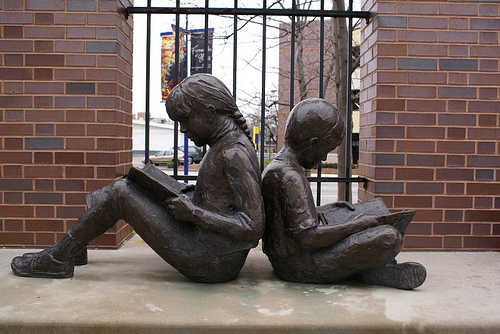
\includegraphics[scale=0.5]{slow_readers.jpg} 

\end{center}
\end{frame}
\end{document}
